% The \phantomsection command is needed to create a link to a place in the document that is not a
% figure, equation, table, section, subsection, chapter, etc.
% https://tex.stackexchange.com/questions/44088/when-do-i-need-to-invoke-phantomsection
\phantomsection

% https://tex.stackexchange.com/questions/5076/is-it-possible-to-keep-my-translation-together-with-original-text
\chapter{\lang{Introduction}{Introdução}}
\phantomsection

{\lang{
    Additive manufacturing (AM) has gained attention for the last two decades for its great potential
    to reduce the time between ideation and production of complex geometries. This characteristic is
    being frequently explored among researchers and engineers to evaluate and compare product concepts
    beyond virtual models and prior to investing in tooling for mass production. The reduced supply
    chain, also has an enormous potential to decrease the lead time between a sales order and the
    delivery of a functional component, consequently reducing inventory cost \cite{VOLPATO2017}.
  }
  {}
}

{\lang{
    Other great potentials of the technology are the reduction of geometric constraints, removing
    barriers to the production of components optimized for multi-physics restrictions and the possibility
    to repair components. These characteristics combined can result in lower assembly part count and
    component weight, as well as cheaper maintenance, leading to lifetime cost reduction, more efficient
    operation and less fuel consumption in systems such as airplanes \cite{ZHANG2017148}.
    \autoref{fig_ma_examples} illustrates applications of different AM technologies used in the aerospace industry.
  }
  {}
}

\begin{figure}[htb]
  \caption{
    \lang{
      Examples of additive manufacturing of metallic components. (a) LBM-produced Ti-6Al-4V bracket
      for Airbus A350 with topology optimized bionic design resulting in ~30 weight saving cp.
      to conventional milled bracket \cite{LIU2017351}. (b) Turbine housing fabricated by the LASERTEC
      65 3D System using multi-axis deposition. (c) Exhaust duct fabricated using the Laser Engineered
      Net Shape (LENS) process \cite{LIU2017351}. (d) Repairing for damaged titanium blisk \cite{SABOORIetAll2019}.
    }{
      Exemplos de manufatura aditiva de componentes metálicos
    }
  }  \label{fig_ma_examples}
  \centering
  \begin{subfigure}{0.24\textwidth}
    \label{fig_ma_examples_a}
    \centering
    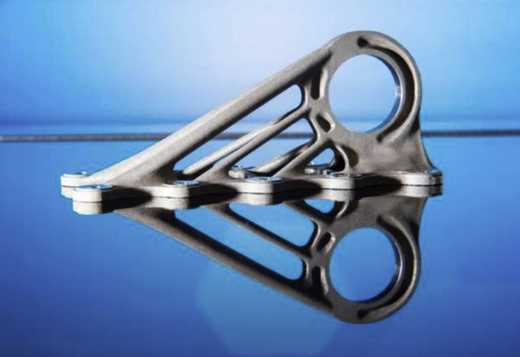
\includegraphics[width=\textwidth]{airbus_bracket_a.png}
    \caption{}
  \end{subfigure}
  \hfill
  \begin{subfigure}{0.24\textwidth}
    \label{fig_ma_examples_b}
    \centering
    \adjincludegraphics[trim=0 {.38\height} 0 0,clip,width=\textwidth]{turbine_housing_b.png}
    \caption{}
  \end{subfigure}
  \hfill
  \begin{subfigure}{0.24\textwidth}
    \label{fig_ma_examples_c}
    \centering
    \adjincludegraphics[trim=0 0 0 {.25\height},clip,width=\textwidth]{exhaust_duct_c.png}
    \caption{}
  \end{subfigure}
  \hfill
  \begin{subfigure}{0.24\textwidth}
    \label{fig_ma_examples_d}
    \centering
    \adjincludegraphics[trim=0 {.15\height} 0 {.15\height},clip,width=\textwidth]{titanium_blisk_repair_d.png}
    \caption{}
  \end{subfigure}
  \hfill

\end{figure}

{\lang{
  Despite the promising features, AM is still expensive when compared to other manufacturing processes,
  especially for processing metals, with only a few technologies applicable to manufacture dense
  components. To accomplish that, Powder Bed Fusion (PBF), Sheet Lamination (SL) and Directed Energy
  Deposition (DED) are some of the AM groups of process available, each one presenting particular
  strengths and limitations \cite{VOLPATO2017}.
}
{}
}

{\lang{
  Among the above mentioned categories, Directed Energy Deposition Laser with Powder as feedstock
  material (DED-LP), a sub category of DED processes, offers advantages such as suitability to repair
  failed components, suitability to produce larger parts with higher build rates when compared to PBF
  technology and the potential to manufacture components with variations in alloy composition along
  the build volume, an advanced class of materials known as Functionally Graded Materials (FGM) \cite{VOLPATO2017}
  \cite{DEBROYetAll2018112}. On the other hand PBF technology offer much better geometry resolution,
  design freedom and enhanced mechanical properties, being one of the most widespread metal manufacturing
  processes \cite{LEWANDOWSKIandSEIFI2016}\cite{FRAZIER2014}.
}
{}
}

{\lang{
  Although some authors argue that the production cost will drop as technology evolves, manufacturing
  metal components by AM is still only justifiable when a significant reduction in lead time, inventory
  cost, part weight or part count takes place \cite{BOURELLetAl2009}. Furthermore, the lack of diffuse
  knowledge of process dependent geometry limitations and output material properties, restrict the choice
  of manufacturing process according to the availability of material data still in the design phase
  \cite{ASHBY2011xi}.
}
{}
}

{\lang{
  In this context, the mechanical properties resulting from the process are of special interest given
  the fact that metals are extensively used to withstand the mechanical loads of a variety of
  applications. Information extracted from stress-strain curves such as Young’s modulus (E), elastic
  limit (Sy) and tensile strength (Su) are the baseline information for the mechanical design of
  structural components as illustrates \autoref{fig_material_information}.
}
{}
}


\begin{figure}[htb]
  \caption{
    \lang{
      Types of material information. Structured data for design “allowables” and the characteristics
      of a material that relate to its ability to be formed, joined, and finished; records of experience
      with its use; and design guidelines for its use \cite{ASHBY2011xi}.
    }{
      Tipos de informação do material.
    }
  }  \label{fig_material_information}
  \centering
  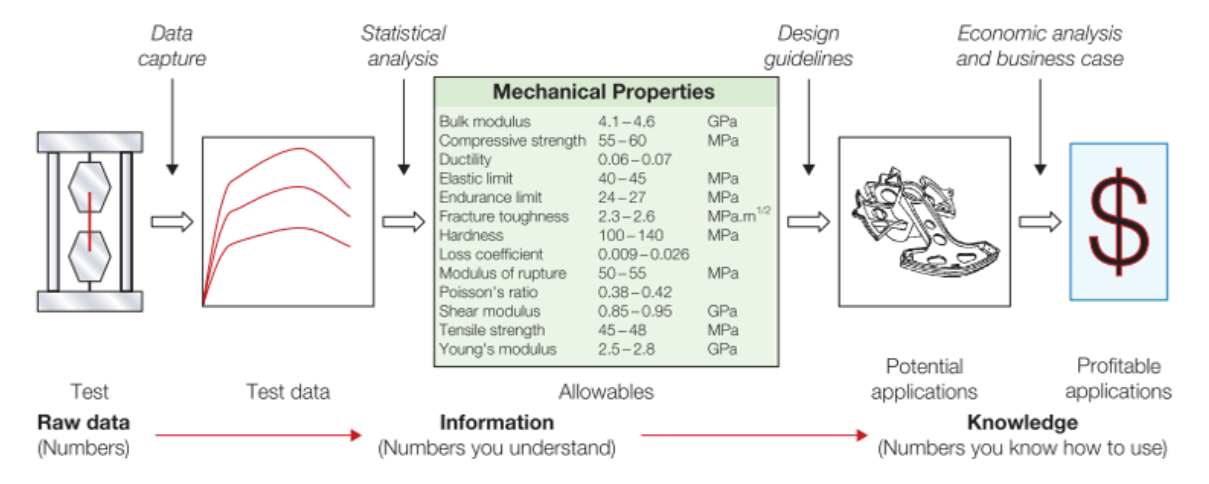
\includegraphics[width=\textwidth]{types_of_material_information.png}
\end{figure}

{\lang{
  Even though an enormous effort has been made for the last decade in order to standardize manufacturing
  practices and data reporting on mechanical properties, a collective understanding of the AM design
  paradigm as well as a database of material properties for different processing conditions is still
  required in order to democratize the technology \cite{BOURELLetAl2014}\cite{BOURELLetAl2009}.
}
{}
}


